\documentclass{sig-alternate}
\usepackage[latin1]{inputenc}
\usepackage[caption=false]{subfig}
\usepackage{url}

%Sacado del paper de Fergu

\begin{document}
%
% --- Author Metadata here ---
\conferenceinfo{GECCO'13,} {July 6--10, 2013, Amsterdam, The Netherlands.}
\CopyrightYear{2013}
\crdata{978-1-4503-1963-8/13/07}
\clubpenalty=10000
\widowpenalty = 10000

\title{Improving Evolutionary Solutions to the Game of MasterMind
  Using an Entropy-based Scoring Method}

%\subtitle{[Extended Abstract]
%\titlenote{A full version of this paper is available as
%\textit{Author's Guide to Preparing ACM SIG Proceedings Using
%\LaTeX$2_\epsilon$\ and BibTeX} at
%\texttt{www.acm.org/eaddress.htm}}}
%
% You need the command \numberofauthors to handle the 'placement
% and alignment' of the authors beneath the title.
%
% For aesthetic reasons, we recommend 'three authors at a time'
% i.e. three 'name/affiliation blocks' be placed beneath the title.
%
% NOTE: You are NOT restricted in how many 'rows' of
% "name/affiliations" may appear. We just ask that you restrict
% the number of 'columns' to three.
%
% Because of the available 'opening page real-estate'
% we ask you to refrain from putting more than six authors
% (two rows with three columns) beneath the article title.
% More than six makes the first-page appear very cluttered indeed.
%
% Use the \alignauthor commands to handle the names
% and affiliations for an 'aesthetic maximum' of six authors.
% Add names, affiliations, addresses for
% the seventh etc. author(s) as the argument for the
% \additionalauthors command.
% These 'additional authors' will be output/set for you
% without further effort on your part as the last section in
% the body of your article BEFORE References or any Appendices.

\numberofauthors{2}
\author{
\alignauthor
J.J. Merelo, Pedro Castillo, Antonio Mora\\
       \affaddr{University of Granada}\\
       \affaddr{GeNeura, Department of Computer Architecture and Technology, ETSIIT + CITIC}\\
       \affaddr{18071 - Granada}\\
       \email{jmerelo,pedro,amorag@geneura.ugr.es}
\alignauthor
Anna I. Esparcia-Alc�zar\\
\affaddr{S2 Grupo}\\
\email{aesparcia@s2grupo.es}
}

\maketitle

\begin{abstract}
Solving the MasterMind puzzle, that is, finding out a hidden
combination by using hints that tell you how close some strings are to
that one is a combinatorial optimization problem that becomes
increasingly difficult with string size and the number of symbols used
in it. Since it does not have an exact solution, heuristic methods
have been traditionally used to solve it; these methods scored each
combination using a heuristic function that depends on comparing all
possible solutions with each other. In this paper we first optimize
the implementation of previous evolutionary methods used for the game
of mastermind, obtaining up to a 40\% speed improvement over
them. Then we study the behavior of an entropy-based score, which has
previously been used but not checked exhaustively and compared with
previous solutions. The combination of these two strategies obtain
solutions to the game of Mastermind that are competitive, and in some
cases beat, the best solutions obtained so far. All data and programs
have also been published under an open source license. 
\end{abstract}

% A category with the (minimum) three required fields
\category{H.4}{Information Systems Applications}{Miscellaneous}
%A category including the fourth, optional field follows...
\category{G.1.6}{Mathematics of Computing}{NUMERICAL ANALYSIS}[Optimization]


%sures, performance measures
\terms{Algorithms}

\keywords{games, evolutionary algorithms, optimization, puzzles}


%
%%%%%%%%%%%%%%%%%%%%%%%%%%%%%%%   INTRODUCTION   %%%%%%%%%%%%%%%%%%%%%%%%%%%%%%%
%
\vfill\eject
\section{Introduction and State of the Art}
\label{sec:intro}
%

Mastermind \cite{wiki:mm,Knuth,Widenius,Montgomery} is a puzzle in which one player $A$ hides a combination of
$\kappa$ symbols and length $\ell$ that the other player $B$ has to
discover by playing combinations coded in the same alphabet and with the same
length.  The answers from player $A$ to every combination include the number of
symbols in the combination that are in the correct position (usually
represented in the actual board game as {\em black} pins) and the
number of symbols that have been guessed correctly but are in a
different position ({\em white} pins). Player $B$ then
makes a new guess and obtains another answer; this process continues until
the hidden one is played by $B$; $B$ then receives as score the number of guesses
made; obviously, higher {\em score} is worse. $A$ and $B$ then interchange their positions. Eventually,
the scores are tallied and the one with the smaller number of guesses
made wins.  In the actual board game, symbols in the alphabet take the
shape of colored pins; that is why we usually talk about {\em colors}
instead of symbols. Historically, the  game which is actually played
by humans \cite{wiki:mm} uses
$\kappa=6$ symbols (or colors) and length $\ell=4$, with {\em Super Mastermind} versions with up
to $\ell=5$ pegs and $\kappa=8$ different colors. 

Solving this kind of puzzle is an exciting endeavor, because  it is a game in which almost any
computer strategy can beat a human, which use a very different
strategy \cite{laughlin1982selection,hubalovsky2012modeling} to play it. But the interesting
part is that solutions to
Mastermind can be applied easily to other games such as MineSweeper
\cite{legendre2012minesweeper} or Hangman since the structure of the game is the
same: probing a part of the search space by making a guess and getting a response from
whoever holds the secret. But its applications are not reduced to
other puzzles or games; solutions to Mastermind have also been used in
the following applications:\begin{itemize}
\item Focardi  \cite{focardi2011guessing} describes a method  to break
  ATMs guessing PINs via making requests to the application
  programming interface of the so-called HSM (hardware security
  modules) which are in charge of encryption in several phases of ATM transactions.
\item Gagneur and coauthors \cite{gagneur2011selective} describe its application
in a procedure called {\em selective phenotyping}. Since it's
impossible to find out the phenotype of a single gene, the only way of
doing it is via phenotyping of several groups of genes that include
the one we are interested in. The procedure  used to find this groups
of combinations of genes is in fact identical to the solution of the
game of Mastermind.
\item Mastermind can be used as a testbed for search algorithms, as
  claims the title of a paper by O\'Geran et
  al. \cite{o1991mastermind}. Strategies developed for Mastermind can
  be applied to other search algorithms as well.
\item Querying player $B$ for how close is the played combination to
  the hidden one and getting an answer is an example of {\em
    information leakage} \cite{chen2011auditing}, since $A$ reveals some info about its
  structure which can be eventually used to find it when enough
  information is available. This technique has been used to find out
  information about particular DNA codes belonging to a particular
  person, in what has been named {\em Mastermind} attack on genomic
  data \cite{goodrich2009mastermind,goodrich2012mtdna}.
 \end{itemize}

Being able to come up with an effective solution that can be applied
to all these problems is a good enough reason, but the generalized
Mastermind problem is also interesting from a theoretical point of
view, with several studies pointing to the fact that it is NP-Hard problem
\cite{DBLP:journals/corr/abs-1111-6922}. The issue of finding bounds to
the number of guesses needed is still open, although Doerr and Winzen
have lately improved in previously found (and rather loose, \cite{Chvatal}) bounds
\cite{doerr2012playing,doerr2012bb}. However, experimental methods are
very far from those bounds, obtaining the solution in a much lower
number of guesses; they are valuable, however, to give a hint on the
scaling of the solution complexity with the number of symbols and the
length. 

In the absence of exact methods, heuristic solutions such as the one studied
in this paper are, for the time being, the best approaches to solve
this problem; they are also the ones that present a better scalability
and are able to solve the problem to the largest problem size. 
These solutions fall mainly into two different types: exhaustive
(which can only solve versions of the game with a small number of
symbols and length due to memory limitations) and
approximate, which do not use (or at least try not to do it in the
general case) the whole search space. Any of them 
\cite{o1991mastermind,francisstrategies:moo,Berghman20091880,nicso}
seek first  combinations that match the answers made to $B$, and
thus could possible be the hidden code. These combinations are called {\em
    eligible}, {\em possible} or {\em
  consistent}. Those solutions are guaranteed to reduce the search space at
least by one, but obviously every one will yield a different
response from $A$, with one being possible optimal (since the set is
bound to include the hidden combination). The problem is that knowing which one is the best is, a
priori, impossible, and in fact how well any eligible combination will
do can only be guessed. 

How do we measure, them, how well a certain combination is going to
behave? 
% Exhaustive methods
% \cite{Knuth,DBLP:journals/corr/abs-1207-1315} would eliminate all
% non-consistent 
% solutions and play a consistent one, while approximate methods
% would sample the set of consistent solutions and play one of
% them, 
By assigning a {\em score} to every eligible combination (or every
combination the method knows of) which
reflects usually how well it will be able to reduce the search space
once played, with the rationale that a scoring method that reduces
quickly the search space will eventually yield a single eligible
combination, which in the case of exhaustive search will be the hidden
code and in approximate methods will be at least a good
candidate. This score will have to be computed using the only
information available to the method: the (possibly partial) set of all
eligible combinations. This set, besides possibly (surely, in case of
exhaustive search) including the hidden combination, has all the
information available to the method on the hidden combination.

So, to compute these scores, every combination is
compared in turn with the rest of the combinations in the set; the
number of combinations that get every response (there is a limited
amount of possible responses, from no blacks/no whites to $\ell -1$
blacks through all combinations of $\ell-p$ blacks and $p$ whites) is noted. Eventually this results in a
series of {\em partitions} in which the set of consistent combinations
is divided by its {\em distance} (in terms of common positions and
colors) to every other.  So, a {\em partition} is a subset of the set
of eligible combinations. All combinations in the eligible set are
then defined by a list of the number of combinations that would obtain
every possible answer, and are scored according to this list. However,
there will be combinations that will have exactly the same list of
values (and thus be in the same {\em partition}), they will obviously
have the same score since they {\em partition} the set of eligible
combinations in the same way. Whatever scoring function we choose,
there will be a non-empty set of combinations with
the best score; one of the combinations of this set is chosen
deterministically (using lexicographical order, for instance) or
randomly to be played. 

Please note that these are heuristic methods based on expected
outcome. On average, they will work as expected, but even combinations
with the same score will obtain a different result depending, of
course, on which is the actual secret combination. Finding the best
one for a particular size, or even a particular set of combinations,
is an open issue which leaves room for research such as the one
performed in this paper. 

These partitions are used to assign a score to every combination;
several scores have been proposed:\begin{itemize}
\item {\em Worst case} was proposed by Knuth \cite{Knuth} as the first rigorous
  strategy to play Mastermind; combinations are scored according to
  the size of the biggest partition; the bigger, the worse. The
  combination to play is extracted from the set of those with the
  smallest biggest combination. Ties are broken by using the first in
  lexicographical order. 
\item {\em Most parts}, proposed in \cite{Kooi200513}, takes into account only the
  number of non-zero partitions. This was the option used by authors
  such as Merelo et al. \cite{mm:cig} in the area of evolutionary
  algorithms. It is fast to compute but it is not clear what is the
  rationale behind it, other than the fact that unlikely combinations
  (such as those with a single symbol) usually have low scores,
  besides, this score is a first approximation of 
\item {\em Entropy}  which has been used in works such as \cite{Neuwirth,bestavros,mm:ppsn:2010}, computes
  the entropy of partitions, and tries to maximize it. Combinations
  with a high entropy also have a high amount of information, which is
  related to the fact that a guess must try and extract the maximum
  information from the hidden guess. 
\item {\em Expected size} used by \cite{Berghman20091880,irving} tries to
  minimize the expected size; this one is related to the Worst Case
  mentioned in the first item and follows the same rationale: by
  playing the combinations that minimize the expected (as opposed to
  worst, in the case of Knuth) size, the set of eligible combinations
  will be cut down eventually to one. 
\end{itemize}

However, scores are heuristic, so, for the time being and there is no rigorous way of
choosing the best score. Experiments so far show that the best strategies are Most parts and
Entropy, with no distinct advantage, for all problem sizes, of any one
of them
over the others \cite{nicso}; and even so, the best results published
so far use a the Expected Size strategy \cite{Berghman20091880}. In fact,
combinations of them are possible, according to
\cite{DBLP:journals/corr/abs-1207-1315}, but have not, so far, been
proved in problems where a sample of the consistent set is used (as
opposed to the whole set); besides, combining the above mentioned
scores is, in fact, a score, and nothing bars somebody with coming up
with a score different from the set mentioned above with the
constraint that it will still use the same information contained in
the consistent set (or a subset thereof).. Most
strategies, however, concentrate on finding the right size for
minimization of the number of turns. The complexity of the solving
algorithm, however, increases quadratically with the set size, since
it involves comparing every combination with the rest, which
implies that the time needed to find the solution and also number of
evaluations increase too fast with the search space size, resulting in a bad
scaling behavior, so using bounds on the set size has a big impact on
the behavior of the algorithm. 

If any method wants to improve over the state of the art, it has got
to be compared with the paper by Berghman et al. in
\cite{Berghman20091880}. They obtained a system that is able to
find the solution in an average number of moves that is, for all sizes
tested, better than any solution previously published; the number of evaluations
was not published, but time was; this last is difficult to compare
(since software and hardware environment is different) but it will
give at least an order of magnitude (sub-second, seconds, minutes)
with which to compare new methods. Besides being the best solutions
found so far, they were very fast. As a point of fact,  some
researchers have tried to break the  search space with a high
dimension barrier by searching for fast solutions: Khalifa and Yampolsky
\cite{khalifa2011ga} were able to solve the length 8, 12 colors
($\ell=8,\kappa=12$) problem in just 8 seconds, but with an average
number of guesses equal to 25 (vs 20.571 seconds and 8.366 average
number of guesses). This probes than there are other ways to solve the
problem if you are not looking for the best solution, but it is not
the venue we will be pursuing in this paper, where we will try to
beat, at least from the point of view of guesses played.  

We will do so by looking at the problems with this approach: there were many parameters that had to be set for
each size, starting with the first guess and the size of the
consistent set, as well as population size and other evolutionary
algorithm parameters; some parameters are studied, but mainly for the
smallest size, while others, like the size of the sample of the
eligible set or the initial combination, are just mentioned for sizes
bigger than baseline. Changing the eligible set size might lead to
better (and possibly slower) solutions. Besides, as mentioned above,
Expected Size does not obtain good values in exhaustive search
methods, so we will use Entropy to score solutions. And finally, we
will try to optimize our method by profiling the application to
identify bottlenecks and iron them out of the implementation.
The Entropy scoring method has
resulted in good results for the smaller sizes
\cite{DBLP:journals/corr/abs-1207-1315} and \cite{mm:evostar13} but
needs a certain amount of parameter seeking to obtain good results. We
will show that our results are competitive and in some cases better
than those considered state of the art and published by Berghman et
al. \cite{Berghman20091880}. This is a small improvement, but
significant, and since we cannot be sure in advance of what is the
optimal value, it is in fact enough to prove this improvement even if
it is a few percentage points.

The rest of the paper is organized as follows: next we outline the
evolutionary method used to play MasterMind in Section
\ref{sec:evo}. Improvements obtained via profiling are shown in
Section \ref{sec:prof} followed by the results of using Entropy as
scoring method in Section
\ref{sec:entropy}. Finally, we draw some conclusions in the final
Section \ref{sec:conc}.


\section{An evolutionary method for playing MasterMind}
\label{sec:evo}

This paper uses the
method called, simply, {\em Evo}
\cite{evostar,mm:ppsn:2010,mm:cig,DBLP:conf/evoW/GuervosCM11,DBLP:conf/cec/GuervosMC11}
(as in EvoMastermind). This
method, which was  released  as open
source code at CPAN (the Comprehensive Perl Archive Network, available
at a mirror near you)
(\url{http://search.cpan.org/dist/Algorithm-Mastermind/}), is an
evolutionary algorithm that has been optimized for speed and number of evaluations.
Evolutionary algorithms \cite{Zen,Michalewicz,eiben03} are a Nature-inspired search and
optimization method that, modeling natural evolution and its molecular
base, uses a  population of solutions encoded into a data structure
(usually a string, but currently any data structure is used) to find the 
optimal one. Candidate solutions are scored according to its closeness to the optimal
solution (called {\em fitness}) and the whole population evolved by
discarding solutions with the lowest fitness and making those with the
highest fitness reproduce via combination (crossover) and random
change (mutation). It is proved that these algorithms are able, given
enough time and resources, to find {\em good enough} and even
optimal solutions to several problems in engineering
\cite{gecco08:pgarcia} and other fields such as economic forecasting \cite{wcci:bankruptcy}. 

Evo, which is explained extensively in
\cite{DBLP:conf/cec/GuervosMC11}, iterates the evolutionary algorithm
until a prefixed amount of consistent combinations has been found; in
this paper and following \cite{merelo12:gameon} that number has been
fixed to ten.  It uses Most Parts \cite{Kooi200513} to
score consistent combinations, and the {\em distance to consistency}
for non-consistent ones, so that the fitness directs search towards
finding consistent solutions and then towards higher-scoring
solutions. If the number of consistent solutions is below the
threshold, different from and stays so for several generations (fixed
to three), the best combination is played; if no feasible combination
is found for a fixed amount of generations (fixed to 50) the
population resets. This is a last-ditch solution which leads to a high
number of evaluations and, in some cases, to an endless loop or resets
which shows that, for that particular configuration, the evolutionary
algorithm is unable to find a solution. These problems are in part
overcome via endgames \cite{goddard2003computer,DBLP:conf/cec/GuervosMC11}, which
streamline the search for solution via different techniques. 

If we keep the consistent set size fixed we still have some parameters
to set, mainly two related ones: population and tournament size; this
size indicates how many combinations will be compared with each other
before selecting a single one to go to the reproduction pool and
selective pressure increases with its value; with a value such as
eight the probability of a low-fitness combination to be selected is
very low, while with a value equal to 2 (the minimum) there is a
certain probability that those combinations with low rankings will be
selected if they {\em joust} in the tournament with each other. The
relationship among both quantities has been well established by B\"ack
and coworkers in \cite{Back94selectivepressure}.

In this paper we have made several improvements over the published
algorithm. We have profiled the application to improve speed, which
has resulted also in a change of the operators used in the
experiments. Second, we have studied several parameter configurations
to improve at the same time the number of evaluations (which results
also in a speed improvement) and the number of games played. And,
finally, we have used a different scoring method over previous papers
in a attempt to beat, or at least equal, the already published
results. 
%%%%%%%%%%%%%%%%%%  Experiments  %%%%%%%%%%%%%%%%%%%
\section{Profiling for performance enhancement}
\label{sec:prof}

One of the first questions one always has to ask about any new
algorithm or method proposed is whether its implementation is, in
fact, the most efficient possible. Implementation matters, as the
authors of
\cite{DBLP:conf/iwann/MereloRACML11,durlak2008implementation} have
proved. Implementation affects not only same-method speed, but also
gives some insight on what is important and what is not in the method,
allowing a more deep understanding of it. 
%
\begin{figure}[!htb]
\centering
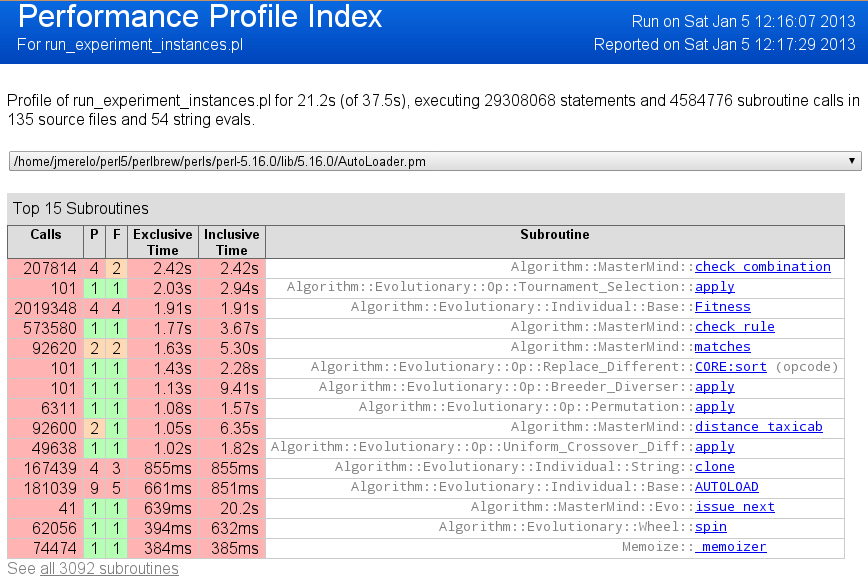
\includegraphics[scale=0.375]{pre-profile.png}
\caption{Output of {\tt Devel::NYTProf} before profiling. Please note
  the place where the algorithm spends most of the time, {\tt
    check\_combination} and, in fact, the top ten functions taking most
  of the time. \label{fig:profile:pre}} 
\end{figure} 
%

Since the code for the methods presented here is written in Perl, we
have used {\tt Devel::NYTProf} a source profiler originally developed
for the New York times. We tested it over 10 runs of the algorithm
with different hidden combinations. Please take into account that,
since evolutionary algorithms are stochastic, there is a certain
amount of randomness in the result. This profiler outputs a file
\footnote{All result files are available under request} that
can be analyzed and output to a set of web pages. The first page of
the report has been captured and is shown in Figure
\ref{fig:profile:pre}.  Prior to this profiling another analysis was
made, it showed that the {\em permutation} operator that converted a
combination in a permutation was extremely slow (since it had to
generate a representation of the combination and proceed to the next
permutation until it reached a random number). That is why it this
operator was eliminated altogether; however, since it is a major
component of the algorithm its effect on performance will be examined
in the next Section. 

This report shows the usual output in profilers, including the number
of calls to a function, exclusive (time spent exclusively in that
function) and inclusive (which includes calls to functions from the
one listed). We usually have to look at the first item, which a
function called {\tt check\_combination}. This is the function that
compares two combinations, be it the hidden combination with the one
played, or obviously more frequently, the combinations in the eligible
set among them or the combinations in the population with the already
played ones to compute fitness. Even as this function had been
optimized in previous versions of the algorithm, it eventually results
that it takes 12$\mu$s per call, which is a lot considering that it is
the core of the algorithm. This makes this function a target for
optimization; however, it is almost impossible to go further using
Perl. It gets worse, however, since this function is called mainly
from the 4th in the list, {\tt check\_rule}, which compares a string
with already played guesses. That adds a few seconds to
the total tally and it gets even worse since this one is called mainly
from {\tt distance\_taxicab}, 9th in the list, where the program spends
almost 70$\mu$s per call, being called almost a hundred thousand times
during the 10 games. This function has been released as an open source
Perl module and is available from CPAN at \url{http://search.cpan.org/dist/Algorithm-MasterMind/}.

That is good news, also, since we have a clear target for
optimization, string comparison. This is the first and most important
optimization performed: {\tt check\_combination} was programmed in C,
and the several levels of indirection used for comparing strings were
reduced when possible. The substitute for {\tt distance\_taxicab} is
called {\tt distance\_xs} (XS is the method for including compiled C
functions inside Perl programs) and is shown at the top of the new
version in Figure \ref{fig:profile:post}.  This new function takes
19$\mu$s per call, less than 1/3 what it did before. Taking into
account that previously it took around 1/3 of the total time, the
total improvement in performance will amount to around 10\%. That is
not dramatic, but since usual experiments take up to several hours, it
might mean a much better turnaround for performing them.

Besides, the optimization does not stop here. The second function is
also an important target for optimization, because it takes a lot of
time and is only called 100 times, one for each generation (around 10
generations per game), and a whooping 29 ms. per call. Since this
function uses lots of complicated data structures it is not such an
easy target for optimization, but still some improvements can be
made. Since most of the time is spent comparing fitnesses, it is just
a matter of substituting a function call ({\tt Fitness()}) by reading
a value ({\tt ->{'\_fitness'}}). It is not a good practice
(implementation might vary), but we trade that for a good increment in
speed (to 5.73 ms. per call); that is basically achieved since that
particular line is called almost a million times during the run. That
can also be seen in the third function in the list, which is
Fitness. By suppressing most calls to that function we inmediately
eliminate its 1.91s from the running time (or at least most of them,
since you actually have to retrieve the fitness). 

Finally, as it happens with most evolutionary algorithms, we find a
sorting function in the sixth place, which is called from many
places. That is specific from the evolutionary algorithm (not
MasterMind) but can be eliminated anyways by using {\tt Sort::Key},
the fastest sort function available in the Perl module repository
(called CPAN). 

%
\begin{figure*}[!htb]
\centering
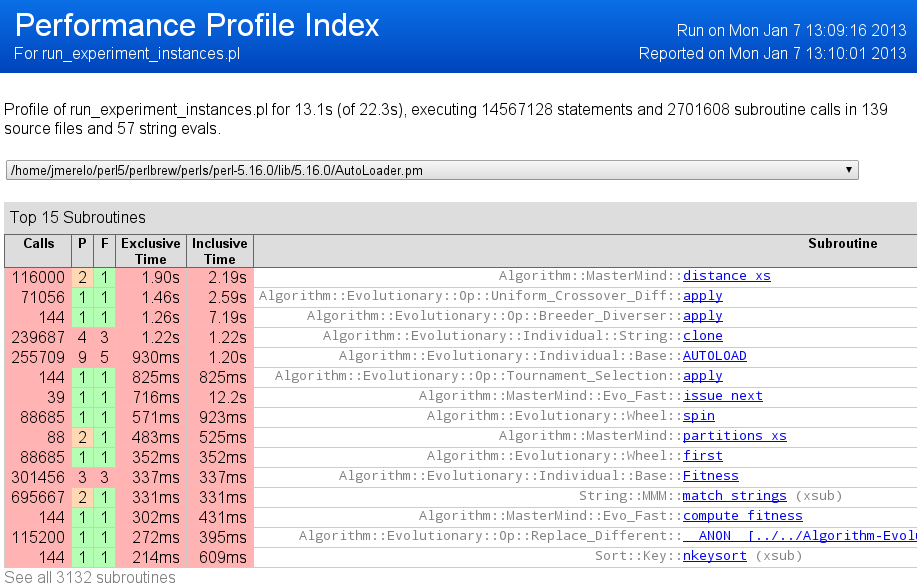
\includegraphics[scale=0.55]{post-profile.png}
\caption{Output of {\tt Devel::NYTProf} after the last optimization
    profiling. The first one now is the new function created, and all
    previously time-hogging functions have
    disappeared. \label{fig:profile:post}} 
\end{figure*} 
%

As we proceed further down the list we could find more convenient
optimizations. However, the effort needed will not result in a big
improvement in speed. Final result for the algorithms eventually used
in this paper are shown in Figure \ref{fig:profile:post}, which now
needs 22.5s to run instead of the previous 37.5, a better than 40\%
improvement in speed. Please note than, even so, the speed of
interpreted languages can be slower than compiled languages. However,
we have proved that big speed improvements can be made by using a
systematic procedure; these speeds can be in many cases much bigger
than those possibly obtained by tweaking or improvement of the
algorithm itself.


\section{Using Entropy for combination scoring in evolutionary MasterMind}
\label{sec:entropy}

\begin{table}[t!]
\centering 
\caption{Values for the Evo parameters that obtain the best
  result. Permutation, crossover and mutation are {\em priorities};
  they are normalized to one to convert them to application rates. In
  practice, crossover will be applied to 80\% and mutation and
  permutation to 10\% of the newly generated combinations each. \label{tab:params}}
\begin{tabular}{lc}
\hline
Parameter & Value \\
\hline \\
Crossover  & 8 \\
Mutation  & 1 \\
Permutation  & 1 \\
Replacement rate  & 0.75 \\ 
\hline
\end{tabular}
\end{table}
%
In this Section we will perform experiments pursuing the two
objectives of this paper: obtain a running time that is competitive
with the state of the art and obtaining better results than those
published in \cite{Berghman20091880}. The new version is called
FastEvoEntropy since its scoring method is Entropy and it is faster
than previously published versions. Two versions of this last method
have been tested: one includes a new permutation operator with a
different implementation that chooses randomly a random number of
characters in the string that shuffles it; the second one substitutes
permutation by two different operators, Shift and Swap; this last one
has been traditionally used by other methods. The first one shifts
with carry a string left or right with the eliminated character being
inserted at the other side; swap is a simple permutation that swaps
the place of two characters (previously checking that they are
different). 

Results for number of guesses (Table \ref{tab:moves}), evaluations
(Table \ref{tab:evals}) and time (Table \ref{tab:time}) are shown. All results
indicate the population and consistent set limit size in parenthesis,
average and error of the mean. Evo++ results are included for the sake
of comparison and were published in \cite{mm:evostar13}; Berghman's
results were published in  \cite{Berghman20091880} when shown (number
of evaluations and, in one case, average time to solution were not
published. In all cases 5000 different games were played; Berghman et
al. cites 500 games in their paper. 

Just two sizes were used for this comparison; they pose a difficult
enough problem for being challenging and, besides, these are the sizes
for which results have been published and can thus be compared against
this new method. The common parameters for all runs are shown in Table
\ref{tab:params}. The rows in each table is correlative, that is, they
correspond to the same experiment. Time measures were not taken
previously so this new Evo version cannot be compared with the
previous one (but the previous Section has sufficiently proved the
former was slower).

\begin{table*}[t!]
\centering
\caption{Comparison among approaches in this paper:  Evo
  and Berghman et al. \cite{Berghman20091880}. Previously obtained results
  published in \cite{mm:evostar13} are also included for the sake of
  comparison. Those labeled EN used Entropy as scoring method, while
  MP use Most Parts. \label{tab:comparison-guesses}}
\subfloat[Mean number of guesses with standard deviation;
the quantities in parentheses indicate population and consistent set
size (in the case of Evo++).]{\label{tab:moves}
\begin{tabular}{lcc}

                    &$\ell=5, \kappa=8$ & $\ell=6,\kappa=9$ \\
\hline
Berghman et al. &             5.618                          & 6.475  \\
\textsc{Evo++ (EN) }   & (1000,200) $ 5.555 \pm 0.011$ & (2000,200) $6.373 \pm 0.011$ \\
\textsc{Evo++ (MP) }   & (1000,80) $ 5.602 \pm 0.012$ & (2000,200) $6.436 \pm 0.012$ \\
\textsc{FastEvoEntropy}   &  (768,32) $ 5.6148 \pm 0.011$ & (1024,32) $6.433 \pm 0.012$ \\
                                               &  (768,256) $ 5.59 \pm 0.012$ &  (1024,256) $6.44 \pm 0.012$ \\
                                               & (1024,256) $5.577 \pm 0.011$ & (2048,256) $6.42\pm 0.012$\\
\textsc{FastEvoEntropy} S+SH & (800, 256) $5.5762 \pm 0.012$ & (1024,256) $6.43 \pm 0.12$\\

\hline
\end{tabular}
}

\subfloat[Mean time to solution with error of the mean;
differences are always significant.]{\label{tab:time}
\begin{tabular}{lcc}

                    &$\ell=5, \kappa=8$ & $\ell=6,\kappa=9$ \\
\hline
Berghman et al. &                                      & 1.284  \\
%\textsc{Evo++ (EN) }   &  $ 26098 \pm 144$ & $67521 \pm 384$ \\
%\textsc{Evo++ (MP) }   & $20120 \pm 114$ & $68860 \pm 406$ \\
\textsc{FastEvoEntropy}   &  (768,32) $ 0.709 \pm 0.004$ & (1024,32) $2.31 \pm 0.93$ \\ 
                                               &  (768,256) $ 3.03 \pm 0.02$ &  (1024,256)  $5.42 \pm 0.034$\\
                                                & (1024,256) $ 3.26 \pm 0.02$ & (2048,256) $6.88 \pm 0.04$ \\
\textsc{FastEvoEntropy} S+SH & (800, 256) $2.93 \pm 0.02 $ &(1024,256)  $5.41 \pm 0.06$ \\
\hline
\end{tabular}
}

\subfloat[Mean number of evaluations with error of the mean;
differences are always significant.]{\label{tab:evals}
\begin{tabular}{lcc}

                    &$\ell=5, \kappa=8$ & $\ell=6,\kappa=9$ \\
\hline
\textsc{Evo++ (EN) }   &  $ 26098 \pm 144$ & $67521 \pm 384$ \\
\textsc{Evo++ (MP) }   & $20120 \pm 114$ & $68860 \pm 406$ \\
\textsc{FastEvoEntropy}    &  (768,32) $ 12679 \pm 73$ &  (1024,32) $38306 \pm 14098$\\
                                                &  (768,256) $ 25167 \pm 141$ & (1024,256) $49492 \pm 288$\\
                                                & (1024,256) $29279 \pm 161$ & (2048,256) $76277 \pm 443$\\
\textsc{FastEvoEntropy} S+SH & (800, 256) $25488 \pm 144 $ & (1024,256) $49663 \pm 779$\\
\hline
\end{tabular}
}


\end{table*}

The tables above show several results. First, the canonical
implementation of the permutation, albeit slow, is better than the new
one, results for Evo++ (EN) are (significantly using Wilcox T-Test)
better than any result published in this paper; this consistently for
the two sizes studied. This issue will have to be pursued further, but
it was not the main objective of this paper, which was to establish a
new state of the art in MasterMind results. 

The results shown in Table \ref{tab:moves} show that, effectively,
this new algorithm is better at solving the game than Berghman's
(incidentally, \cite{mm:evostar13} too). The difference is small but
significant using Wilcoxon t-test, and that is so for all methods
that use 256 as consistent set limit size; for $\ell=6,\kappa=9$, even
when the smaller size (consistent set size CS=32) is used. This new
version of the method, as is usual, achieves the best results with a
sizable population and CS=256. However, increasing more the
population (to 2048) does not result in a noticeable (in fact, not
significantly better) decrease in the number of games needed to win.
We can also notice in the results that the new permutation operator is
not significantly different from the new swap+shift (S+SH) operators;
as already pointed out, both are worse than the canonical permutation
operator. On the other hand, the main conclusion drawn from the
time-to-solution table (\ref{tab:time} is that, in fact, it is
difficult to obtain a solution faster than Berghman's et al. did. You
can obtain a better solution, but not a faster solution. We should
have to improve the faster solution around 50\% to obtain it as fast
as Berghman's. However even if it is a bit slower, it is better. By
reducing even further the CS size and population it it's not
impossible to achieve that target. That, for the moment, is left as
future work. 

The third table with the average number of evaluations show that these
new methods, even achieving worse results, do so using a comparable
number of evaluations (for $\ell=5$) or considerably less (for
$\ell=6$). This is due to the change in the operators used, and also
shows that it is possible that exploration of search space changes
considerably with them and they are unable to find the best solutions
so efficiently. There is also a rough correlation between the number
of evaluations and the time needed to find the solution and some hope
in the fact that, despite the search space for $\ell=6,\kappa=9$
being roughly 30 times larger than $\ell=5, \kappa=8$, since we will
be able to pursue bigger problem spaces with a probably logarithmic
increase in the time. 

Finally using S+SH is a bit faster than using (the new) permutation
operator, as shown in the last row of results. In any case, results
are good enough so the new operators introduced in this work have
proved its worth as alternatives to permutation.

\section{Conclusions}
\label{sec:conc}

In this paper we have tried to establish a new state of the art with a
method that is able to obtain better solutions to the game of
MasterMind than those published and do it in less time. However, we
have not managed to achieve both objectives: our results are better
than those published but considerably slower. There is some room for
improvement in both aspects, but that is left as future work. The
achieved results, however, show a big improvement in the number of
evaluations needed and the time needed to do them, thanks to the
optimization done after profiling the method. This profiling has led
to a change in the algorithm by eliminating a slow operator which,
however, has resulted in worse results than previously obtained. As
indicated above, this is a result that will have to be pursued
further.

The main result, thus, in this paper, which is obtaining a better
player at Mastermind than the state of the art, has been achieved
mainly by using Entropy as a scoring method. Previously
\cite{mm:evostar13} it proved to be better than most parts and both
are known to be better than Worst Case  \cite{Knuth}. However, so far
Expected Case (used by Berghman) obtained the best results. This is no
longer so, and it will have to be explored whether entropy effectively
continues being a good scoring method for eligible combinations when
the size of the search space increases. 

It should be noted also that all results, configuration files and data
are available under an open source licence (address hidden for double
blind revision). 

Several possible lines of work have been pointed out above. Profiling
is a methodology that is obviously valid for a particular problem
size. When size increases new functions may start to be the
bottleneck, so size-specific optimizations are also possible. Another
option is to code in C other critical parts of the program, but none
so simply have been found, so other speedup methods (including
complete factorization) should be sought.

An interesting option that would be worth exploring is using
multi-threaded applications to simulate parallel execution within a
single computer. This will speed up the application, but it will have
an important impact on the algorithm so it will have to be examined
carefully looking at different alternatives and ways of interaction of
the different threads. We think that it is going to be difficult to
obtain much improvement over the average number of games obtained here
(or, for that matter, in other papers pursuing this research issue), even using exhaustive
search when a sufficiently powerful machine is found, so any
improvement on the algorithm will have to be done on the number of
evaluations needed or the time needed to reach them. 

%ACKNOWLEDGMENTS are optional
\section{Acknowledgments}

This work is supported by projects TIN2011-28627-C04-02 awarded by the Spanish Ministry of Science and Innovation and P08-TIC-03903 awarded by the Andalusian Regional Government, as well as CANube, project 83 CEI BioTIC \url{http://biotic.ugr.es}
%
% The following two commands are all you need in the
% initial runs of your .tex file to
% produce the bibliography for the citations in your paper.


%\bibliographystyle{abbrv}
\bibliographystyle{plain}
\bibliography{GA-general,geneura,mastermind}  % sigproc.bib is the name of the Bibliography in this case


\end{document}